\documentclass[english]{article}
\usepackage[T1]{fontenc}
\usepackage[latin9]{inputenc}
\usepackage{babel}
\usepackage{graphicx}
\usepackage{subfigure}
\usepackage{float}
\setlength{\parindent}{0pt}
\usepackage{amsmath}


\begin{document}

\title{Lab 1: Infrared Imaging\\ -------------------------------- \\ \Large Sensors and Digitization}
\author{ \ Armine Vardazaryan, Songyou Peng \\ arminevardazaryan@gmail.com, psy920710@gmail.com}
\date{26th November 2015}

\maketitle

\section{Introduction}
In this laboratory work we studied an infrared imaging system and its properties. 
We used it to measure the temperature of objects. \\
The system comprised a computer and an infrared camera Cedip SC7000 with its software Altair.\\
\section{Defect detection using IR camera}
In this section, after studying how to use the software and creating a project and connecting the camera, we use it to find the hot transistor on a circuit.\\

\begin{figure}[H]
	\centering
	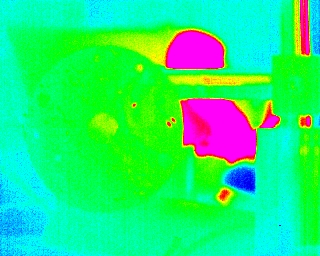
\includegraphics[width=0.3\linewidth]{Pictures/circuit_cold001.JPG}
	\caption{The IR image of the circuit with power off}
	\label{fig:one}
\end{figure}
In the image above the vague shape of the circuit can be seen in green. 
Because the circuit in the image is not connected to the power supply, it can be observed that the temperature appears to be uniform all around the surface of the circuit.\\
However, when the circuit is turned on, we see a region change its color.\\
\begin{figure}[H]
	\centering
	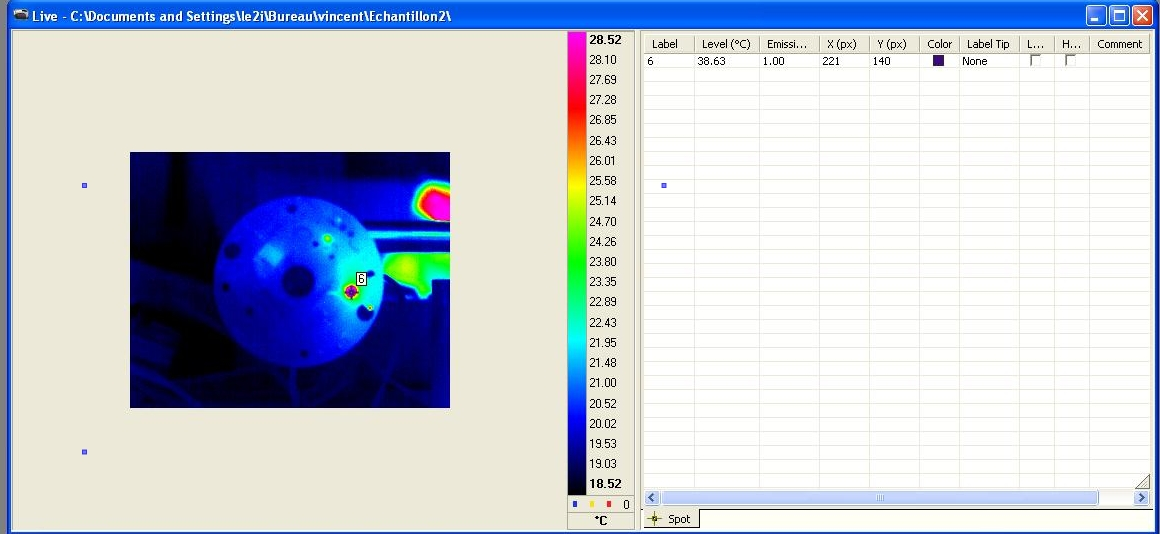
\includegraphics[width=1\linewidth]{Pictures/position1.JPG}
	\caption{The IR image of the circuit with power on}
	\label{fig:two}
\end{figure}
In Figure \ref{fig:two} we see that at position (221, 140) in the view of the camera, the temperature is rising.
We see that the camera measures approximately $39 \textdegree$C.
This value, of course, is not precise because the camera assumes the emissivity of the object to be 1 when, in fact, no real object has emissivity of 1.\\
With this kind of system, we can measure the mean estimated temperature of the whole circuit, as seen in the image below, where we specify the area of interest for the measurement.\\
\begin{figure}[H]
	\centering
	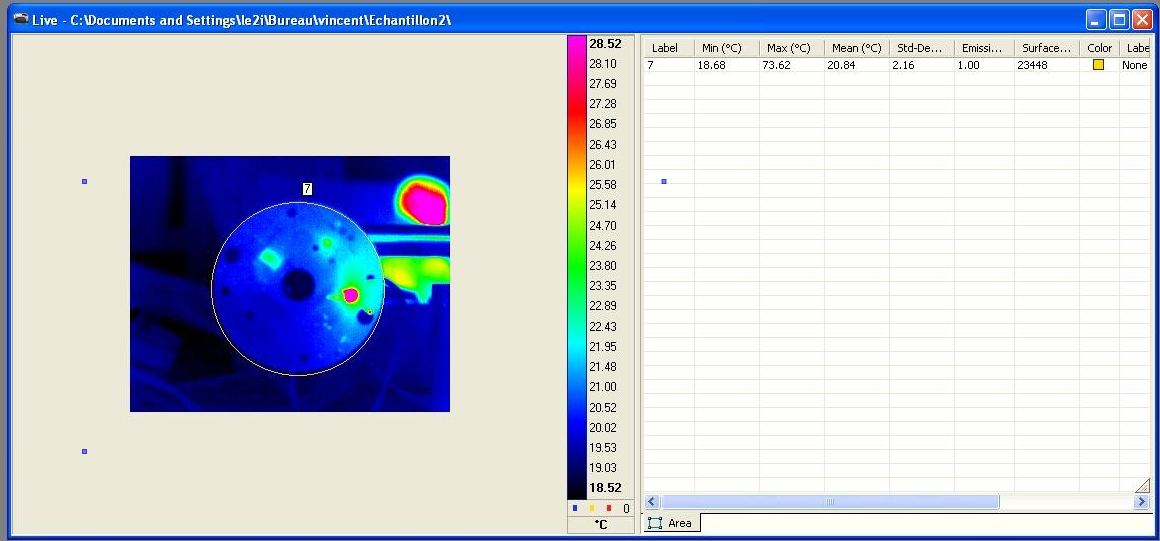
\includegraphics[width=1\linewidth]{Pictures/max1.JPG}
	\caption{Mean temperature measurement of the circuit}
	\label{fig:three}
\end{figure}
Here we can see that the camera estimates the mean temperature of the circuit area to be around $21 \textdegree$C.\\
Another useful measurement that can be done is finding a profile of the temperature along a line on the circuit\\
<image missing?>

\subsection{Wolff's method}


\section{Contrast polarization measurement}
\subsection{Polarizers and a rotator}
\section{Conclusion}

\section{References}
{[}1{]} Wolff, Lawrence B. "Polarization vision: a new sensory approach to image understanding." Image and Vision computing 15.2 (1997): 81-93.\\
{[}2{]} Goldstein, Dennis H. Polarized light. CRC Press, 2010.\\
{[}3{]} -https://en.wikipedia.org/wiki/Polarizer\\


\end{document}